\documentclass[12pt,notitlepage,nofootinbib]{revtex4}
\usepackage{graphicx}
\usepackage{bm}
\usepackage{rotating}
\def\baselinestretch{1.2}
\usepackage{dcolumn}
\usepackage{times}
\usepackage{color}
\usepackage{amsmath,amssymb,amsfonts} 
\usepackage{extarrows}
\usepackage{listings}
\usepackage{url}
\setlength{\mathindent}{0pt}

\begin{document}

\title{StochSS Hands-on Tutorial Series: 4 - Spatial Stochastic Simulations with StochSS}

\author{StochSS Development Team}
\affiliation{Department of Computer Science - University of California, Santa Barbara}

\date{\today}

\maketitle

\section{\label{sec:pre}Prerequisites}
\begin{itemize}
\item StochSS 1.4 (or later) installed on your computer (please follow download and installation instructions at \url{www.stochss.org}). 
\item A basic understanding of well-mixed discrete stochastic simulations and models based on ordinary differential equations \cite{dan,sundials}.
\item A basic knowledge of the mesoscopic reaction-diffusion master equation and of the next sub volume method (NSM) \cite{nsm}.
\item  A basic familiarity with the StochSS GUI (please consult the \textit{Basic Introduction to StochSS} tutorial).
\item The following login screen appears in your browser; please log in.
\end{itemize}

\begin{figure}[!ht]
\centering
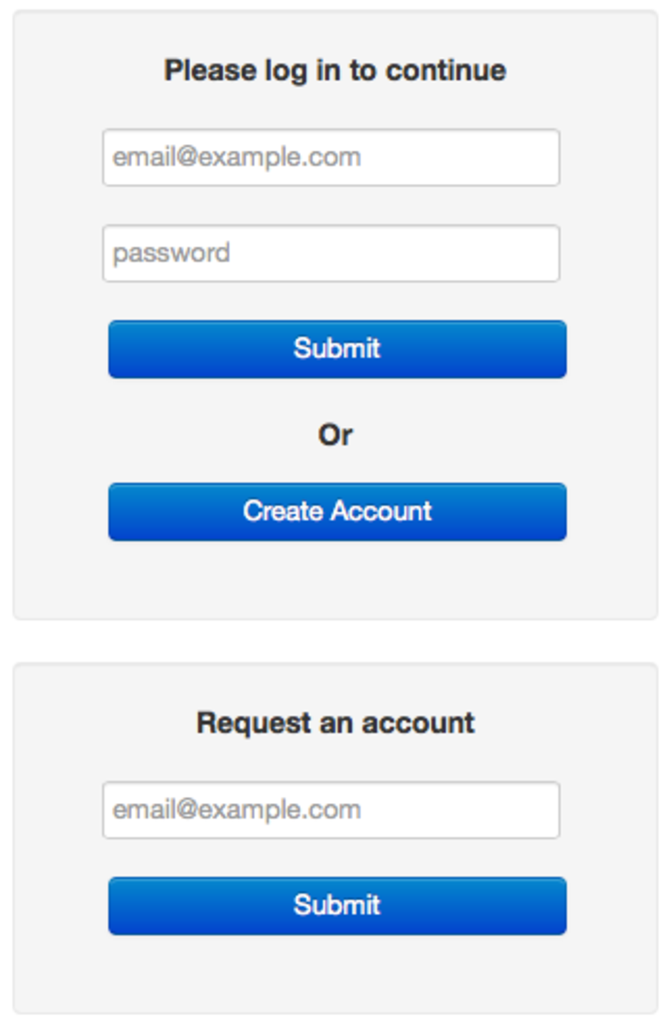
\includegraphics[scale=0.55]{user-login.pdf}
\end{figure}

\newpage

\section{Spatial Stochastic Simulations}
The spatial stochastic simulation capabilities in StochSS are based on PyURDME \cite{urdme}. PyURDME is a general software framework for modeling and simulation of stochastic reaction-diffusion processes on unstructured, tetrahedral (3D) and triangular (2D) meshes. Unstructured meshes allow for a more flexible handling of complex geometries compared to structured, Cartesian meshes. The current core simulation algorithm is based on the mesoscopic reaction-diffusion master equation (RDME) model. The default solver is an efficient implementation of the NSM.

\subsection{An Instructive Example}
We will build a simple model based on an annihilation reaction between two chemical species generated  by sources located at the two opposite bases of an enclosing cylinder.

The creation of our new spatial model using the \textcolor{blue}{Model editor} progresses through the following steps:
\begin{itemize}
\item \textbf{Navigate} to the main \textcolor{blue}{Model editor} (the \textcolor{blue}{`Model'} tag is selected by default).
\item \textbf{Enter} a model name in the \textcolor{blue}{`Name'} text box, select the \textcolor{blue}{`Population'} button and the \textcolor{blue}{`Spatial'} button. Finally, \textbf{click} on the \textcolor{blue}{`Create model'}  button.
 \item \textbf{Click} on the \textcolor{blue}{`Species�} tag to define chemical species names and their diffusion coefficient. 
 \item \textbf{Use} the \textcolor{blue}{`Add species�} button on the right to add \textit{A} and \textit{B} species both with diffusion coefficient $D=1$.
 \item \textbf{Click} on the \textcolor{blue}{`Parameters�} tag to define model parameters names and their expressions. 
 \item \textbf{Use} the \textcolor{blue}{`Add parameter�} button to add parameter \textit{k1} with a value of $100$.
 \item \textbf{Click} on the \textcolor{blue}{`Reactions�} tag to define reaction names, reactants, products and propensities.
 \item \textbf{Use} the \textcolor{blue}{`Add reaction�} button to add reactions \textit{R1, R2, R3} (see Fig.~\ref{fig:2}). To insert reaction R1 and R2 (`birth' reactions) leave the `Reactants' text box empty and type in the name of the generated species in the `Products' text box.
 To define R3 (the annihilation reaction), type in the species names separated by a comma in the 
`Reactants' text box. Leave the `Products' text box empty. Check out the on-screen help buttons.
 \item \textbf{Click} on the \textcolor{blue}{`Mesh�} tag and select `Cylinder'. You will notice that the cylindrical mesh is divided in three subdomains. Select the proper `buttons' in sections 3 and 4 on the `Mesh` page. Keep in mind that species A is generated in subdomain 1, whereas species B is generated in subdomain 3. Both species are allowed to diffuse everywhere within the cylinder (in all three subdomains). In other words, reaction R1 should be limited to subdomain 1 and reaction R2 to subdomain 3. Reaction R3 can happen in all three subdomains.
  \item \textbf{Click} on the \textcolor{blue}{`Add Initial Condition�} button and \textcolor{blue}{`Select�} `Scatter', `A', `Subdomain = 1',`Count = 500'. \textbf{Click} on the \textcolor{blue}{`Add Initial Condition�} again and \textcolor{blue}{`Select�} `Scatter', `B', `Subdomain = 3',`Count = 500'. \textbf{Click} on the \textcolor{blue}{`Add Initial Condition�} button.
\item Your spatial model is completely defined and ready to be simulated.

\item \textbf{Navigate} to the \textcolor{blue}{Simulation manager} page.

\item \textbf{Select} the spatial model you just created and \textbf{click} on the \textcolor{blue}{`Next�} button.
\item \textbf{Setup} your simulation parameters: name, time, data storage frequency and realizations. 
\item To define the initial random seed, \textbf{click} on \textcolor{blue}{`Advanced Settings�}.
\item \textbf{Click} on the \textcolor{blue}{`Run locally' button}.
\item In a few seconds you will be directed to the \textcolor{blue}{Job Status} page where you can check the status of your simulation.
\item Once your simulation is complete, \textbf{click} on the \textcolor{blue}{`View results�} link to open the \textcolor{blue}{Job summary} page where you can visualize the diffusion of the two species (A and B) over time within the cylindrical container and download the simulation�s output files.

\end{itemize}

\begin{figure}[!ht]
\centering
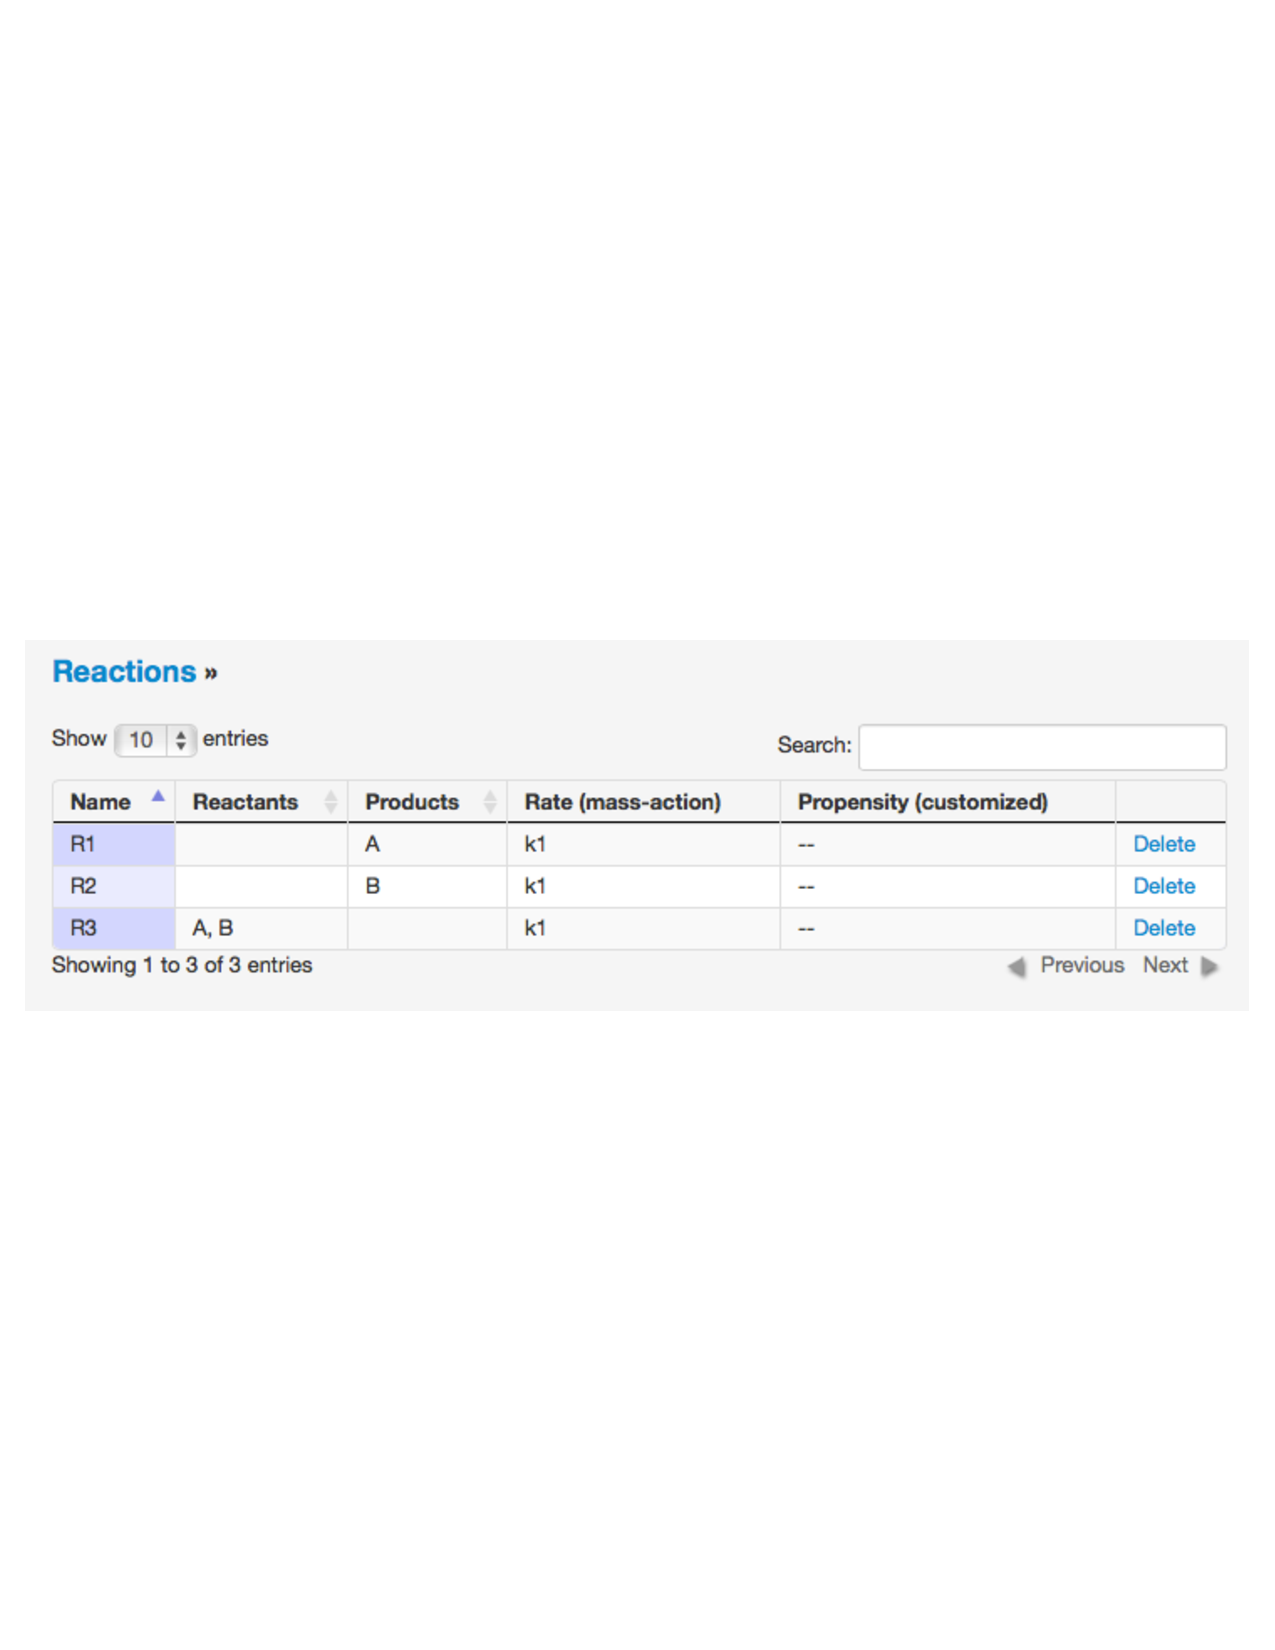
\includegraphics[scale=0.64]{reactions-spatial.pdf}
\caption{`Reactions' page}
\label{fig:2}
\end{figure}

\newpage

\begin{thebibliography}{9}
  
  \bibitem{dan}
  D.T. Gillespie.
  \textit{Exact stochastic simulation of coupled chemical reactions}.
  J. Phys. Chem., 81(25), 2340-2361 (1977)
  
  \bibitem{sundials}
  A. C. Hindmarsh et al.,
  \textit{SUNDIALS: Suite of nonlinear and differential/algebraic equation solvers}.
  ACM Trans. Math. Softw., 31(3), 363-396 (2005)
  
  \bibitem{nsm}
  J. Elf and M. Ehrenberg,
  \textit{Spontaneous separation of bi-stable biochemical systems into spatial domains of opposite phases} IEEE Systems Biology, 1, 230�6 (2004)
  
 \bibitem{urdme}
 B. Drawert, S. Engblom and A. Hellander, 
 \textit{URDME: {A} modular framework for stochastic simulation
of reaction-transport processes in complex geometries}. BMC Systems Biology, 6, 76 (2012)
  
\end{thebibliography}

\end{document}
